% \clearpage
\begin{docCommand}{tcbox}{\oarg{options}\marg{box content}}
  
Creates a colored box which is fitted to the width of the given \meta{box content}. 
In principle, most \meta{options} for a \refEnvLe{tcolorbox}
can be used for |\tcbox| with some restrictions. 
A |\tcbox| cannot have
a lower part and cannot be broken.

% 创建一个盒子, 适应给定的\meta{box content}的宽度。%
% 原则上, 大部分用在 \refEnvLe{tcolorbox} 上的 \meta{options},用在 |\tcbox| 上时有一些限制。%
% 比如,|\tcbox| 没有lower部分,也不能分页。

创建一个彩色的盒子,它适应于给定的\meta{box content}的宽度。原则上,大多数\refEnvLe{tcolorbox}的\meta{选项}都可以用于|\tcbox|,但有一些限制。|\tcbox| 不能有下部分,也不能被分割。
\begin{dispExample}
\tcbset{colframe=blue!50!black,colback=white,colupper=red!50!black,
        fonttitle=\bfseries,nobeforeafter,center title}

Text \tcbox{你好} \tcbox[tcbox raise base]{世界}\hfill
%
\tcbox[left=0mm,right=0mm,top=0mm,bottom=0mm,boxsep=0mm,
  toptitle=0.5mm,bottomtitle=0.5mm,title=我的表格]{%
  \arrayrulecolor{blue!50!black}\renewcommand{\arraystretch}{1.2}%
  \begin{tabular}{r|c|l}
  一   & 二    & 三 \\\hline\hline
  语   & 数   & 英 \\\hline
  理 & 化 & 生
  \end{tabular}}\hfill
%
\tcbox[colback=blue!85!black,
  left=0mm,right=0mm,top=0mm,bottom=0mm,boxsep=1mm,arc=0mm,boxrule=0.5pt,
  title=我的图片]{%
  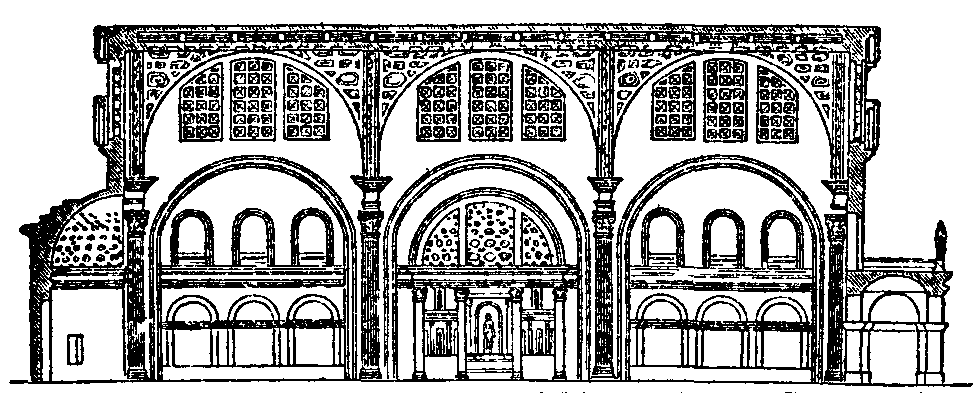
\includegraphics[width=5cm]{Basilica_5.png}}
\end{dispExample}

\begin{带标题示例}{你好哇!}
\begin{调用系统命令的例子}{}
\PassOptionsToPackage{no-math}{fontspec}
\PassOptionsToPackage{AutoFakeBold=true,AutoFakeSlant=true}{xeCJK}
\documentclass{book}
\usepackage[heading=true
,scheme=chinese
,fontset=none
,space=auto
]{ctex}
\setCJKmainfont{方正书宋_GBK}
\setCJKsansfont{方正黑体简体}
\setCJKmonofont{方正书宋简体}

\usepackage[all]{tcolorbox}
\begin{document}
\thispagestyle{empty}
\tcbset{nobeforeafter}
Text \tcbox{你好} \tcbox[tcbox raise base]{世界}\hfill
\end{document}
\end{调用系统命令的例子}
\end{带标题示例}

%a

\begin{dispExample}
% \usepackage{tikz}
\tcbset{colframe=blue!50!black,colback=white,colupper=red!50!black,
        fonttitle=\bfseries,center title}

% 固定宽度的盒子
\begin{tcolorbox}tcolorbox中\\可以使用换行命令!\end{tcolorbox}

% 宽度自适应盒子 (类似 hbox 、 makebox)
\tcbox{tcbox中\\换行命令\newline 无效的情况!}

% 宽度自适应盒子 (使用 \tikzname\  node)
\tcbox[tikznode]{你好\\tikznode可以换行!}
\end{dispExample}

\end{docCommand}

% \clearpage
\begin{marker}
See \Vref{subsec:xparse_tcolorbox} and \Vref{subsec:xparse_tcbox} for more
elaborate methods to create new environments and commands.

参见 \Vref{subsec:xparse_tcolorbox} 和 \Vref{subsec:xparse_tcbox} 了解更多创建新环境和命令的方法。%详细阐述
\end{marker}